\documentclass[11pt,a4paper]{article}
\usepackage[utf8]{inputenc}
\usepackage{amsmath,amsfonts,amssymb}
\usepackage{graphicx}
\usepackage{geometry}
\geometry{margin=1in}
\usepackage{booktabs}
\usepackage{hyperref}
\usepackage{float}
\usepackage{xcolor}

\definecolor{darkbg}{HTML}{0d121f}
\definecolor{lighttext}{HTML}{e2e8f0}
\definecolor{primary}{HTML}{8b5cf6}
\definecolor{secondary}{HTML}{0dd5c5}
\definecolor{accent}{HTML}{10b981}

\pagecolor{darkbg}
\color{lighttext}

\hypersetup{
    colorlinks=true,
    linkcolor=secondary,
    urlcolor=secondary,
    citecolor=accent
}

\title{\textbf{EE3621: Digital Signal Processing} \\ \Large Student Lecture Notes — Lecture 24 \\ \large Design of IIR Filters from Analog Filters — Impulse Invariance}
\author{III B.Tech EEE — Core Exam Preparation Guide}
\date{}

\begin{document}

\maketitle

\noindent\rule{\textwidth}{0.5pt}

\section{Core Concept of Impulse Invariance}

\subsection{Definition \& Invariance Criterion}
The \textbf{Impulse Invariance Method} designs a digital IIR filter by sampling the continuous-time impulse response $h_a(t)$ of an analog prototype filter at uniform sampling intervals $T_s$:
\begin{equation}
\mathbf{h[n] = T_s \, h_a(n T_s)}, \quad n = 0, 1, 2, \dots
\end{equation}
The factor $T_s$ scales the discrete response so that the digital filter's low-frequency gain matches the analog filter.

\subsection{The Fundamental Pole Mapping Rule}
Let the analog filter transfer function be expanded in partial fractions with distinct poles $s_k$:
\begin{equation}
H_a(s) = \sum_{k=1}^N \frac{A_k}{s - s_k} \iff h_a(t) = \sum_{k=1}^N A_k e^{s_k t} u(t)
\end{equation}
Sampling at $t = n T_s$ and taking the $Z$-transform yields the \textbf{Master Operational Formula}:
\begin{equation}
\mathbf{\frac{A_k}{s - s_k} \quad \xrightarrow{\quad \text{Impulse Invariance} \quad} \quad \frac{T_s A_k}{1 - e^{s_k T_s} z^{-1}}}
\label{eq:master_ii}
\end{equation}
Every continuous pole at $s = s_k$ maps directly to a discrete pole at:
\begin{equation}
\mathbf{z_k = e^{s_k T_s}}
\end{equation}

\noindent\rule{\textwidth}{0.5pt}

\section{Stability Mapping \& The Aliasing Dilemma}

\subsection{Preservation of Stability}
Let an analog pole be $s_k = \sigma_k + j\Omega_k$. The corresponding digital pole has magnitude:
\begin{equation}
|z_k| = |e^{(\sigma_k + j\Omega_k)T_s}| = e^{\sigma_k T_s}
\end{equation}
\begin{itemize}
    \item If $\sigma_k < 0$ (Left-Half $s$-Plane) $\implies |z_k| = e^{\sigma_k T_s} < 1$ (\textbf{Inside the Unit Circle}).
    \item \textbf{Theorem:} A stable analog filter is **always mapped into a strictly stable digital filter**.
\end{itemize}

\subsection{Frequency Relationship \& The Aliasing Problem}
The normalized digital frequency $\omega$ is related to analog frequency $\Omega$ by:
\begin{equation}
\omega = \Omega T_s
\end{equation}
The discrete frequency spectrum is an infinite periodic superposition of shifted analog spectra:
\begin{equation}
H(e^{j\omega}) = \sum_{k=-\infty}^\infty H_a\left(j\frac{\omega - 2\pi k}{T_s}\right)
\end{equation}
Because the analog rational transfer function $H_a(j\Omega)$ cannot be strictly band-limited to $|\Omega| \le \pi/T_s$, the high-frequency tails fold back into the baseband $[-\pi, \pi]$, creating **aliasing distortion**.

\begin{figure}[H]
\centering
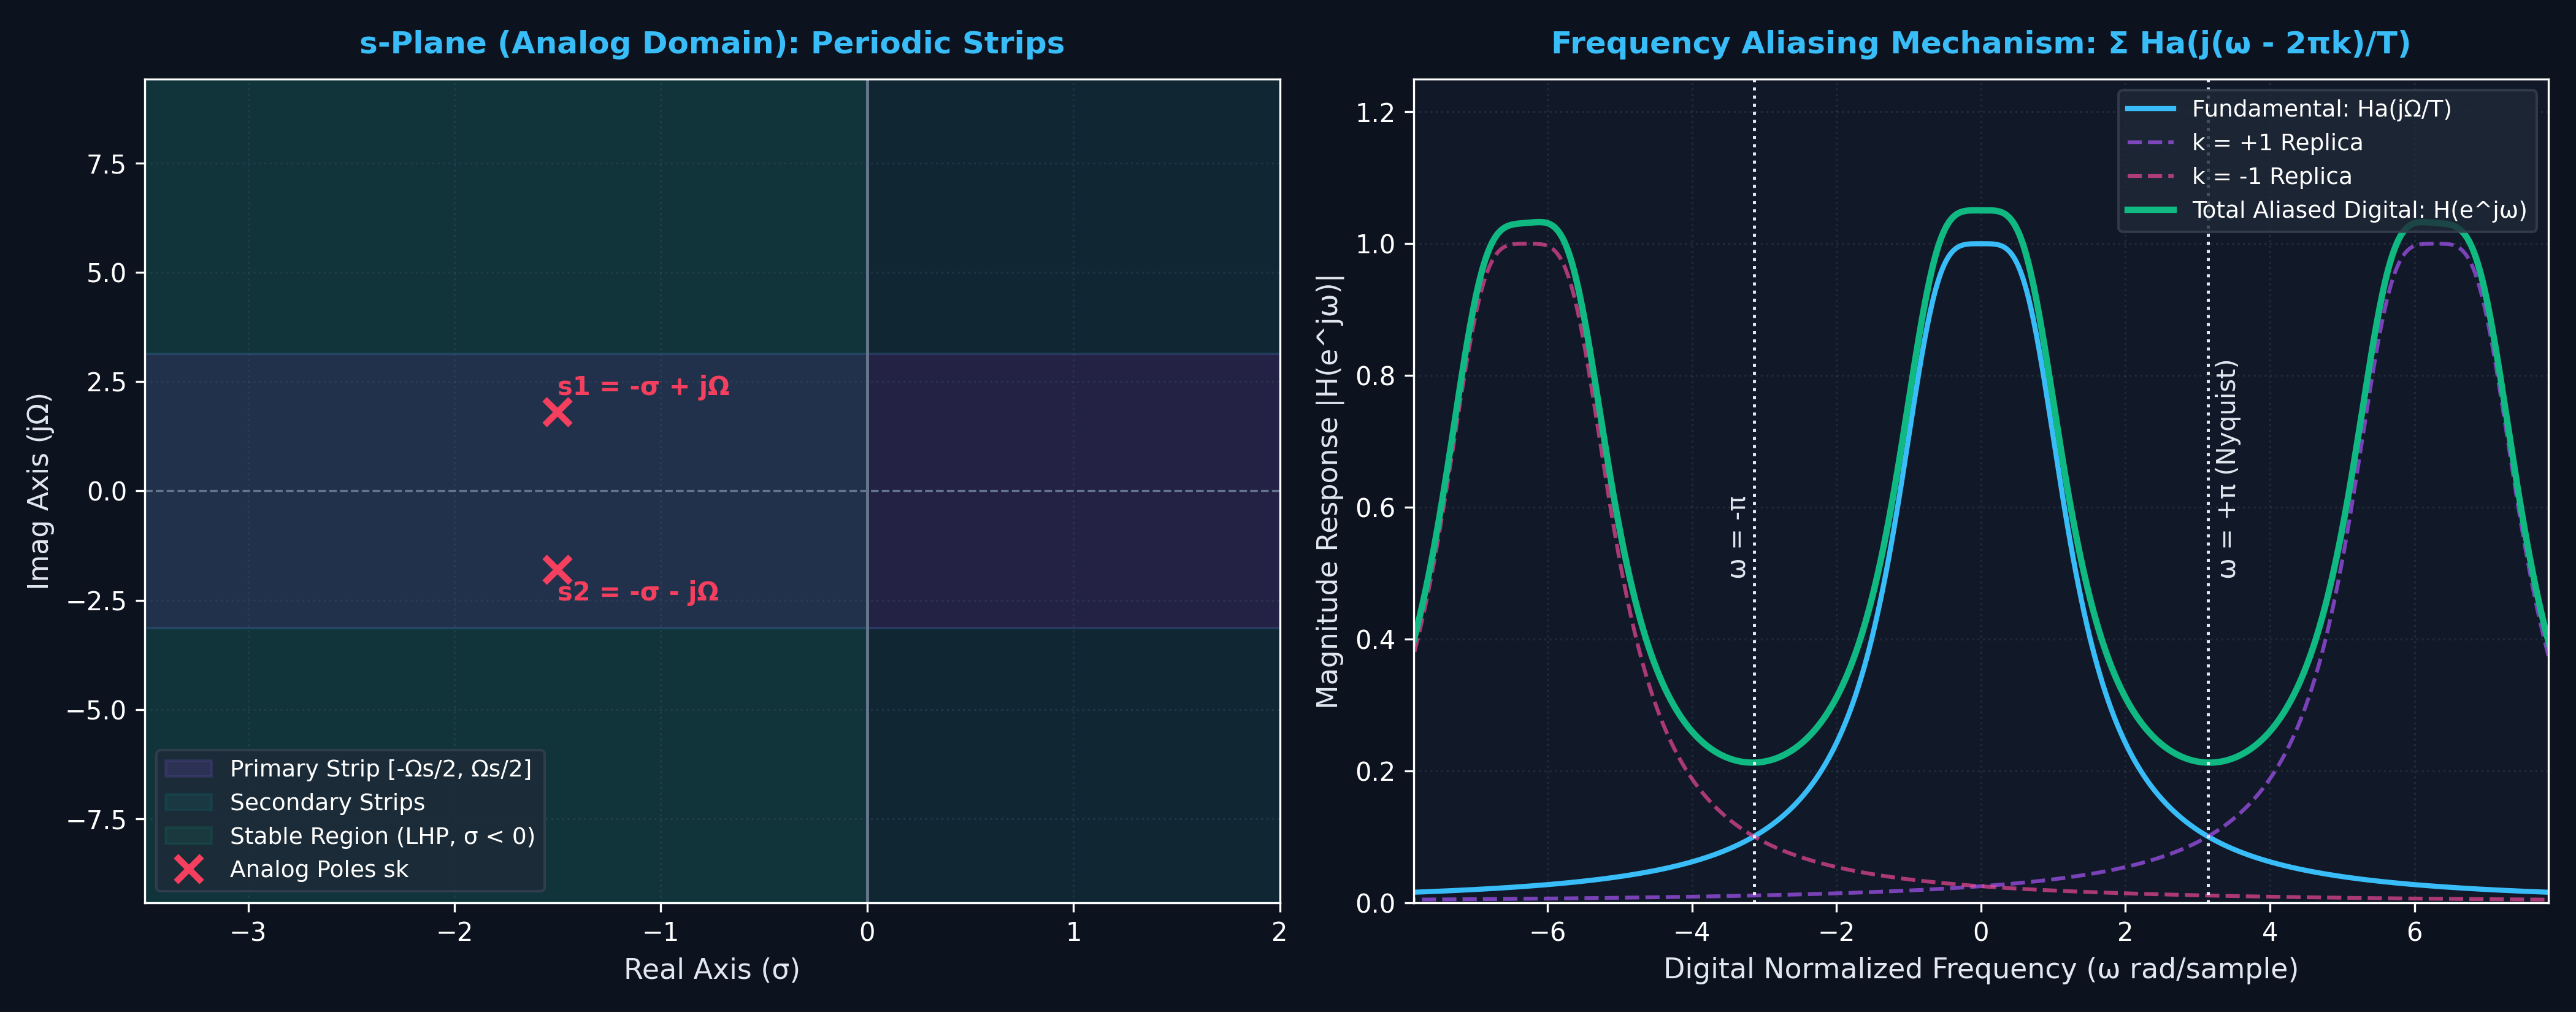
\includegraphics[width=0.75\textwidth]{images/iir_impulse_invariance_mapping.png}
\caption{Left: Horizontal strips of width $2\pi/T_s$ in the $s$-plane mapping into the $z$-plane unit circle. Right: Aliasing caused by overlapping tails of the periodic spectrum copies.}
\label{fig:ii_aliasing}
\end{figure}

\begin{itemize}
    \item \textbf{Suitable Filters:} Lowpass and Bandpass filters whose analog stopband attenuates deeply ($> 30\text{--}40$ dB) at the Nyquist frequency $\Omega_N = \pi/T_s$.
    \item \textbf{Unsuitable Filters:} Highpass and Bandstop filters \textbf{CANNOT be designed} via impulse invariance because their high-frequency gains fold over into DC ($\omega = 0$), destroying stopband attenuation.
\end{itemize}

\noindent\rule{\textwidth}{0.5pt}

\section{Step-by-Step Design Protocol}

\begin{enumerate}
    \item \textbf{Identify Sampling Interval $T_s$ and Frequencies:} Convert digital specifications using $\Omega = \omega / T_s$.
    \item \textbf{Factor the Analog Transfer Function:} Find all poles $s_k$ of $H_a(s)$.
    \item \textbf{Perform Partial Fraction Expansion:}
    \begin{equation}
    H_a(s) = \sum_{k=1}^N \frac{A_k}{s - s_k}, \quad \text{where } A_k = \lim_{s \to s_k} (s - s_k) H_a(s)
    \end{equation}
    \item \textbf{Apply Pole Mapping Formula:} Replace each term by $\frac{T_s A_k}{1 - e^{s_k T_s} z^{-1}}$.
    \item \textbf{Combine Conjugate Terms:} Put complex conjugate pole pairs over a common quadratic denominator to yield real biquad filter coefficients.
\end{enumerate}

\noindent\rule{\textwidth}{0.5pt}

\section{Standard Solved Exam Example}

\textbf{Problem:} An analog second-order Butterworth lowpass filter with cutoff $\Omega_c = 1$ rad/s is given by:
\begin{equation}
H_a(s) = \frac{1}{s^2 + \sqrt{2} s + 1}
\end{equation}
Design the corresponding digital IIR filter using the Impulse Invariance method with $T_s = 1$ second.

\vspace{1mm}
\noindent\textbf{Solution:}

\noindent\textbf{Step 1: Find the Analog Poles}
\begin{equation}
s^2 + \sqrt{2} s + 1 = 0 \implies s_{1,2} = -\frac{1}{\sqrt{2}} \pm j \frac{1}{\sqrt{2}} \approx -0.7071 \pm j 0.7071
\end{equation}

\noindent\textbf{Step 2: Partial Fraction Expansion}
\begin{equation}
H_a(s) = \frac{A_1}{s - s_1} + \frac{A_2}{s - s_2}
\end{equation}
Evaluating the residues:
\begin{equation}
A_1 = \frac{1}{s_1 - s_2} = \frac{1}{j 2(0.7071)} = \frac{1}{j \sqrt{2}} = -j \frac{1}{\sqrt{2}} \approx -j 0.7071
\end{equation}
and $A_2 = A_1^* = +j \frac{1}{\sqrt{2}} \approx +j 0.7071$.

\noindent\textbf{Step 3: Map Poles to the Z-Domain ($T_s = 1$ s)}
\begin{equation}
z_1 = e^{s_1 T_s} = e^{-0.7071 + j 0.7071} = e^{-0.7071}\angle(0.7071 \text{ rad})
\end{equation}
Converting $0.7071 \text{ rad} = 0.7071 \times \frac{180^\circ}{\pi} \approx 40.51^\circ$:
\begin{equation}
e^{-0.7071} \approx 0.4931, \quad \cos(40.51^\circ) \approx 0.7602, \quad \sin(40.51^\circ) \approx 0.6496
\end{equation}
\begin{equation}
z_1 = 0.4931(0.7602 + j 0.6496) \approx \mathbf{0.3748 + j 0.3203}, \quad z_2 = z_1^* = \mathbf{0.3748 - j 0.3203}
\end{equation}

\noindent\textbf{Step 4: Combine into Real Second-Order Biquad}
\begin{align}
H(z) &= \frac{T_s A_1}{1 - z_1 z^{-1}} + \frac{T_s A_2}{1 - z_2 z^{-1}} = \frac{-j \frac{1}{\sqrt{2}}(1 - z_1^* z^{-1}) + j \frac{1}{\sqrt{2}}(1 - z_1 z^{-1})}{(1 - z_1 z^{-1})(1 - z_1^* z^{-1})} \nonumber \\
     &= \frac{j \frac{1}{\sqrt{2}}(z_1^* - z_1) z^{-1}}{1 - 2\text{Re}(z_1) z^{-1} + |z_1|^2 z^{-2}}
\end{align}
Evaluating the numerator and denominator parameters:
\begin{itemize}
    \item $z_1^* - z_1 = -j 2\text{Im}(z_1) = -j 2(0.3203) = -j 0.6406$
    \item Numerator coefficient: $j \frac{1}{\sqrt{2}}(-j 0.6406) = \frac{0.6406}{\sqrt{2}} \approx \mathbf{0.4530}$
    \item Denominator $z^{-1}$ coefficient: $2\text{Re}(z_1) = 2(0.3748) = \mathbf{0.7496}$
    \item Denominator $z^{-2}$ coefficient: $|z_1|^2 = (0.4931)^2 \approx \mathbf{0.2431}$
\end{itemize}
The final digital filter transfer function is:
\begin{equation}
\mathbf{H(z) = \frac{0.4530 z^{-1}}{1 - 0.7496 z^{-1} + 0.2431 z^{-2}}}
\end{equation}
Stability verification: Poles are at $r = |z_{1,2}| = 0.4931 < 1$, ensuring a strictly stable digital filter.

\noindent\rule{\textwidth}{0.5pt}

\section{Essential Exam Checklist \& Traps}
\begin{itemize}
    \item[$\square$] \textbf{Partial Fraction Rule:} Always expand $H_a(s)$ into partial fractions first. Never substitute $s = \frac{1}{T}\ln(z)$ algebraically into $H_a(s)$.
    \item[$\square$] \textbf{The Scaling Factor $T_s$:} Always include $T_s$ in the numerator: $\frac{T_s A_k}{1 - e^{s_k T_s} z^{-1}}$.
    \item[$\square$] \textbf{Zero Locations:} Remember that **zeros do not map** via $z = e^{s T_s}$. Only poles obey this mapping.
    \item[$\square$] \textbf{Highpass Prohibition:} Impulse Invariance cannot be used to design Highpass filters due to infinite spectral foldover (aliasing) at DC.
\end{itemize}

\end{document}
